\bb
\ii Define $T\colon \R^3\rightarrow \R^3$ to be reflection through the plane $\mathcal{P}\colon x+y+z=0$. In other words, $T$ takes an input $(x,y,z)$ and sends it to its reflection $(x',y',z')$ on the other side of $\mathcal{P}$. You may take it on faith that $T$ is a linear transformation. 
\bb
\ii Draw a picture of $\mathcal{P}$, an arbitrary point $(x,y,z)$, and its reflection $(x',y',z')$. Add some right triangles to your picture to indicate the relation between $(x,y,z)$ and $(x',y',z')$. 
\ii Pick a {\em nonstandard} basis $B'$ of $\R^3$, for which the behavior of $T$ is easy to determine: i.e., pick a basis that reflects the geometry of this picture. Compute $[T]_{B'}$. 
\ee 
\begin{solution}
\noindent
(a) In general to draw the reflection of a point $P=(x,y,z)$ through a plane $\mathcal{P}$, draw the line $\ell$ passing through $(x,y,z)$ that is perpendicular to $\mathcal{P}$ (so parallel to its normal vector), and call its intersection with the plane $Q$. (If you recall, $Q$ is just the projection of $P$ onto $\mathcal{P}$. The reflection of $P$ is then the point $P'$ on $\ell$ on the other side of $\mathcal{P}$, whose distance to $Q$ is equal to the distance from $P$ to $Q$. If $P$ is in the plane to begin with, then it is equal to its own reflection. 
\[
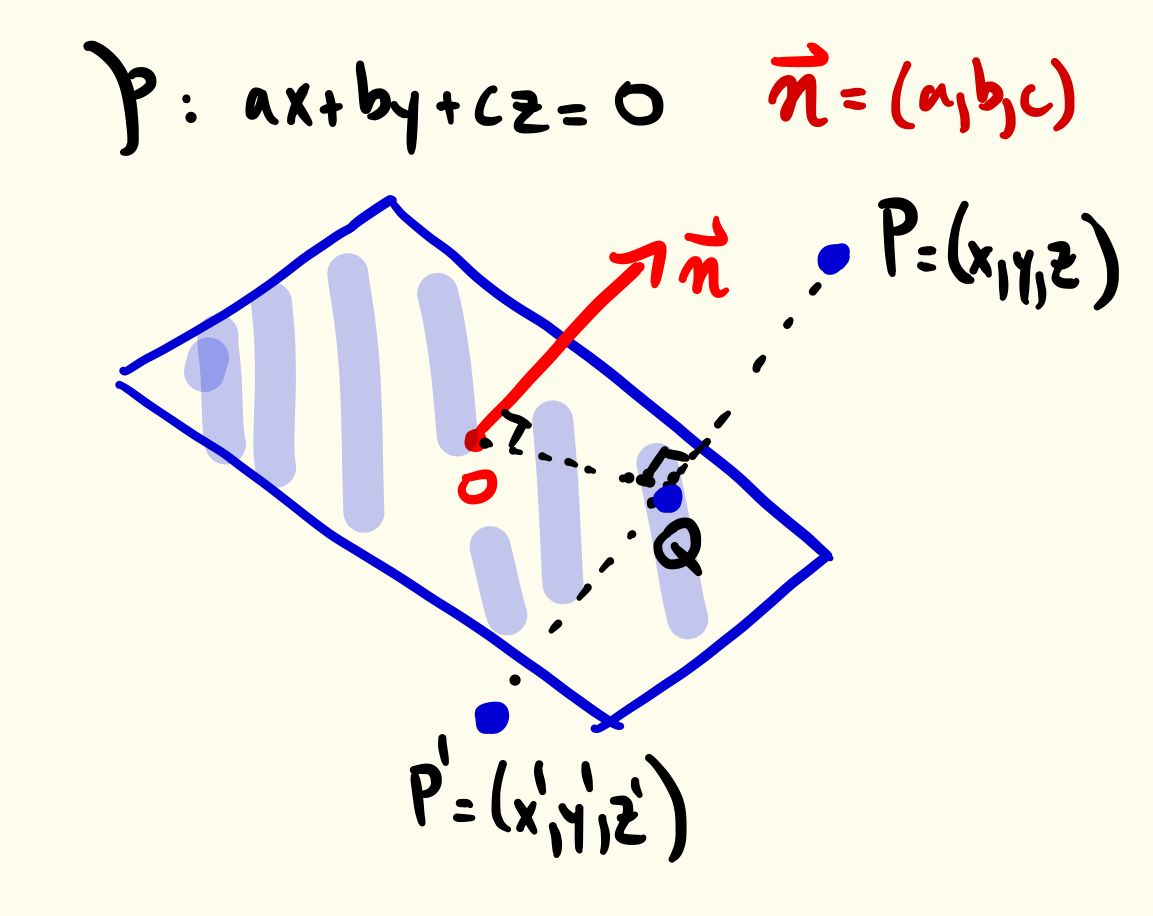
\includegraphics[width=4in]{../Lectures/Images/ReflectionThroughPlane}
\]
(b) The description above helps us pick a basis $B$ of $\R^3$ that makes $[T]_B$ particularly simple. Start of by choosing a basis $\{\boldv_1, \boldv_2\}$ for the given plane $\mathcal{P}$: in our case, the vectors $\boldv_1=(1,-1,0), \boldv_2=(0,1,-1)$ will do. To extend this to a full basis of $\R^3$, we add the normal vector $\boldn$ to the plane. In our case, the basis is thus $B=\{\boldv_1=(1,-1,0), \boldv_2=(0,1,-1), \boldn=(1,1,1)\}$. 

Now, we have $T(\boldv_1)=\boldv_1$ and $T(\boldv_2)=\boldv_2$, since $\boldv_1$ and $\boldv_2$ lie in the plane already. Furthermore, from the picture we describe in (a) it is clear that $T(\boldn)=-\boldn$. This is because the projection of $\boldn$ onto the plane is just $\boldzero$; so its reflection is just $-\boldn$. 

Lastly we now easily compute the coordinate vectors of these outputs: $[T(\boldv_1)]_B=[\boldv_1]_B=(1,0,0), [T(\boldv_2)]_B=[\boldv_2]_B=(0,1,0)$, and $[T(\boldn)]_B=[-\boldn]_B=(0,0,-1)$. We conclude that 
\[
[T]_B=\begin{bmatrix}
1&0&0\\
0&1&0\\
0&0&-1
\end{bmatrix}.
\]

\end{solution}
\ii Consider the differential equation 
\[
f''(x)+f'(x)=x^2+x+1 \tag{$*$}
\]

The theory of ODE's tells us that there are infinitely many solutions $f(x)$ to $(*)$. We will use linear algebra to find infinitely many polynomial solutions. 
\bb
\ii First define $T\colon P_{3}\rightarrow P_{2}$ as $T(f)=f''(x)+f'(x)$. Explain why $T(f)$ indeed lies in $P_2$ and show that $T$ is linear. 
\ii Compute $A=[T]_{B}^{B'}$ where $B$ and  $B'$ are the standard bases of $P_{3}$ and $P_{2}$, respectively. 
\ii Determine $\NS(A)$ and $\CS(A)$. 
\ii Find all solutions in $P_3$ to the differential equation $(*)$. (First solve the relevant matrix equation involving $A$, then ``lift up" to $P_3$. )
\ee
{\footnotesize Note: though we have found all {\em polynomial solutions} to the differential equation $(*)$, we have not found {\em all} solutions. Observe that $g(x)=e^{-x}$ is a solution to the corresponding homogeneous equation $f''+f'=0$, It follows from basic ODE theory that we can add $ce^{-x}$ to any of our solutions in (d) to get a new solution. Our analysis didn't catch these solutions as we restricted our attention to $P_3$. }
\\
\begin{solution}
\ \\(a) The usual proof shows $T$ is linear. Since taking the derivative knocks down the degree of a polynomial by 1, it's clear that if $p(x)$ has degree at most $3$, then $T(p)=p''+p'$ will have degree at most $2$.

(b) Let $B=\{1,x,x^2,x^3\}$ and $B'=\{1, x, x^2\}$. The usual recipe for $[T]_{B',B}$ begins by computing 
\[
T(1)=0, T(x)=1, T(x^2)=2+2x, T(x^3)=6x+3x^2.
\] 
Taking coordinate vectors with respect to $B$ and placing these in columns yields 
\[
A=\begin{bmatrix}
0&1&2&0\\
0&0&2&6\\
0&0&0&3
\end{bmatrix}.
\]
(c) The rank of $A$ is clearly 3 (look at rows), and by inspection we see that $\{(1,0,0), (2,2,0), (0,6,3)\}$ is a basis for $\CS(A)$. Since $\dim\CS(A)=3$ and $\CS(A)\subset\R^3$, it follows from the Subspace Dimension Theorem that $\CS(A)=\R^3$.

Since $\rank(A)=3$, it follows from R-N that $\nullity(A)=4-3=1$. To come up with a basis for $\NS(A)$ we simply need to find one nonzero element of $\NS(A)$. We see $\{(1,0,0)\}$ does the trick. 

What does all this mean about $T$? Since $\CS(A)=\R^3$, it follows that $\range(T)=P_2$. Thus for {\em any} $q(x)\in P_2$, we can find a $p(x)\in P_3$ with $T(p)=p''(x)+p'(x)=q(x)$. This means not only can we solve the given differential equation, we can solve any similar equation of the form $f''+f'=q$, where $q$ is a polynomial in $P_2$.  

Furthermore, as we will see, the fact that $\NS(A)$ is nontrivial will mean that we can always find infinitely many solutions to $(*)$. 

(d) The polynomial $x^2+x+1$ corresponds via $[\hspace{8pt}]_{B'}$ to the vector $\begin{bmatrix}1\\ 1\\ 1\end{bmatrix}$. All solutions $\boldx$ to
\[
A\boldx=\begin{bmatrix}1\\ 1\\ 1\end{bmatrix}
\] 
will lift up to the solutions $p$ to $T(p)=x^2+x+1$. 

Using GE, we see the general solution to the matrix equation is 
\[
\boldx=c\begin{bmatrix}1 \\ 0 \\ 0 \end{bmatrix}+\begin{bmatrix}1\\-\frac{1}{2}\\ \frac{1}{3} \end{bmatrix}
\]
Thus the general {\em polynomial} solution to the original differential equation is 
\[
p(x)=c+(1-\frac{1}{2}x^2+\frac{1}{3}x^3)=(c+1)-\frac{1}{2}x^2+\frac{1}{3}x^3.
\]

\end{solution}
\ii Define $T\colon M_{22}\rightarrow M_{22}$ by $T(A)=A^T-A$. 
\bb
\ii Compute $A=[T]_B$ where $B$ is the standard basis for $M_{22}$. 
\ii Compute bases for $\NS(A)$ and $\CS(A)$.
\ii Use your result in (b) to give bases for $\NS(T)$ and $\range(T)$. 
\ii Identify $\NS(T)$ and $\range(T)$ as familiar subspaces of matrices. 
\ee
\begin{solution}
\ \\
(a) The usual recipe yields 
\[
A=\begin{bmatrix}[rrrr]0&0&0&0\\
0&-1&1&0\\
0&1&-1&0\\
0&0&0&0
\end{bmatrix}.
\]
We have $\NS(A)=\Span(\{(1,0,0,0), (0,0,0,1), (0,1,1,0)\}$ and $\CS(A)=\Span(\{(0,-1,1,0)\}$. 

By lifting we get that 
\[
\NS(T)=\Span\left(\left\{\begin{bmatrix}[rr] 1&0\\ 0&0\end{bmatrix}, \begin{bmatrix}[rr] 0&0\\ 0&1\end{bmatrix}, \begin{bmatrix}[rr]0&1\\ 1&0 \end{bmatrix}\right\}\right), \ \range(T)=\Span\left(\left\{\begin{bmatrix}[rr] 0&-1\\ 1&0\end{bmatrix}\right\}\right).
\]
From these descriptions it follows easily that $\NS(T)$ is the subspace of all symmetric matrices, and $\range(T)$ is the subspace of all skew-symmetric matrices. 
\end{solution}
\ii Let $T:P_2\rightarrow P_3$ be the linear transformation defined by $T(p)=x\cdot p(x-3)$. 
\bb
\ii Find $[T]_{B}^{B'}$ relative to the bases $B=\{1,x,x^2\}$ and $B' = \{1,x,x^2,x^3\}$.
\ii Use $[T]_{B}^{B'}$ to compute bases for $\NS T$ and $\range T$. 
\ee
\begin{solution}
\noindent By the formula for $T$
\begin{eqnarray*}
T(1) &=& x(1) = x\\
T(x) &=& x(x-3) = x^2 - 3x\\
T(x^2) &=& x^3-6x^2+9x
\end{eqnarray*}
Taking these vectors relative the the basis $B'$, we can write
$$
[T]_{B}^{B'} = 
\begin{bmatrix}[ccc]
0&0&0\\
1&-3&9\\
0&1&-6\\
0&0&1
\end{bmatrix}
$$
\end{solution}
\ii Let $T:P_2 \rightarrow M_{22}$ be the linear transformation defined by
$$
T(p) =
\begin{bmatrix}[cc]
p(0)&p(1)\\
p(-1)&p(0)
\end{bmatrix}
$$
let $B$ be the standard basis for $M_{22}$, let $B'=\{1,x,x^2\}$ and $B''=\{1,1+x,1+x^2\}$ be bases for $P_2$. 
\bb
\ii Find $[T]_{B'}^{B}$ and $[T]_{B''}^{B}$.
\ii Use either one of the matrix representations from (a) to compute bases for $\NS T$ and $\range T$. 
\ee
\begin{solution}
\noindent Lets work on $[T]_{B}^{B'}$ first. By the formula for $T$
\begin{eqnarray*}
T(1) &=&
\begin{bmatrix}[rr]
1&1\\
1&1
\end{bmatrix}\\
T(x) &=&
\begin{bmatrix}[rr]
0&1\\
-1&0
\end{bmatrix}\\
T(x^2) &=&
\begin{bmatrix}[rr]
0&1\\
1&0
\end{bmatrix}\\
\end{eqnarray*}
Taking these vectors relative the the basis $B$, we can write
$$
[T]_{B}^{B'} =
\begin{bmatrix}[rrr]
1&0&0\\
1&1&1\\
1&-1&1\\
1&0&0
\end{bmatrix}
$$
Now for $[T]_{B}^{B''}$. By the formula for $T$
\begin{eqnarray*}
T(1) &=&
\begin{bmatrix}[rr]
1&1\\
1&1
\end{bmatrix}\\
T(1+x) &=&
\begin{bmatrix}[rr]
1&2\\
0&1
\end{bmatrix}\\
T(1+x^2) &=&
\begin{bmatrix}[rr]
1&2\\
2&1
\end{bmatrix}\\
\end{eqnarray*}
Taking these vectors relative the the basis $B$, we can write
$$
[T]_{B}^{B''} =
\begin{bmatrix}[rrr]
1&1&1\\
1&2&2\\
1&0&2\\
1&1&1
\end{bmatrix}
$$
\end{solution}
\ii Let $T:M_{22} \rightarrow R^2$ be the linear transformation given by
$$
T\left(
\begin{bmatrix}[rr]
a&b\\
c&d
\end{bmatrix}
\right)
= 
\begin{bmatrix}[cc]
a+b+c\\
d
\end{bmatrix}
$$
and let $B$ be the standard basis for $M_{22}$, $B'$ be the standard basis for $R^2$ and let
$$
B'' = \left\{
\begin{bmatrix}[c]
1\\
1
\end{bmatrix},
\begin{bmatrix}[c]
-1\\
0
\end{bmatrix}
\right\}
$$
be another basis for $R^2$. Find $[T]_{B}^{B'}$ and $[T]_{B}^{B''}$.
\\
\begin{solution}
\noindent By the formula for $T$, we can find $T(\boldu_i)$ where $\boldu_i$ are the vectors in the basis $B$.
\begin{eqnarray*}
T(\boldu_1) &=& 
\begin{bmatrix}[c]
1\\
0
\end{bmatrix}\\
T(\boldu_2) &=& 
\begin{bmatrix}[c]
1\\
0
\end{bmatrix}\\
T(\boldu_3) &=& 
\begin{bmatrix}[c]
1\\
0
\end{bmatrix}\\
T(\boldu_4) &=& 
\begin{bmatrix}[c]
0\\
1
\end{bmatrix}
\end{eqnarray*}
Taking these vectors relative the the basis $B'$, we can write
$$
[T]_{B}^{B'} =
\begin{bmatrix}[rrrr]
1&1&1&0\\
0&0&0&1
\end{bmatrix}
$$
Taking these vectors relative the the basis $B''$, we can write
$$
[T]_{B}^{B''} =
\begin{bmatrix}[rrrr]
0&0&0&1\\
-1&-1&-1&1
\end{bmatrix}.
$$
\end{solution}
\ee